\section{Change Points Detection}

Both for the murders dataset and for the diachronic analysis of the newspaper corpus the time series show abrupt changes in their statistical properties. In the language of time series analysis, these points are called \textbf{change points}, and detecting them is a crucial step in understanding the underlying dynamics of the data.

Many algorithms exist for change point detection \cite{truongSelectiveReviewOffline2020}: in the case of \textit{offline change points detection} the optimal approach is given by the \textbf{Pruned Exact Linear Time} (PELT) algorithm \cite{killickOptimalDetectionChangepoints2012}, which is able to find the optimal segmentation of a time series in linear time, given a cost function and a penalty for adding more change points. The algorithm is very flexible, as it allows for different choices of cost functions; moreover, it's very efficient (linear time complexity), making it suitable for large datasets.

One crucial part of change-point detection with PELT is the choice of the penalty term, which controls the trade-off between the goodness of fit and the number of change points detected. While some methods exists for choosing the penalty (e.g., BIC, AIC) \cite{truongSelectiveReviewOffline2020}, a more robust approach is given by measuring the number of change points detected as a function of the penalty value: on this idea are based the \textit{slope heuristics} \cite{baudrySlopeHeuristicsOverview2012} and the \textit{CROPS} algorithm \cite{haynesEfficientPenaltySearch2014}.

Our approach for choosing the penalty is instead based on the idea of \textit{random shuffling}: by randomly permuting the time series multiple times and applying PELT on each shuffled version of the data, it's possible to obtain an estimate of the number of change points that would be detected by chance for a given penalty value. 
In practice, the optimal penalty value is found by identifying the point where the number of change points detected on the shuffled data drops to zero.

While a python package for changepoint detection is readily available in Python \cite{truongSelectiveReviewOffline2020}, for this specific task I needed a fast implementation of the PELT algorithm that could handle multiple runs efficiently and in parallel. Thus, I developed a python package that implements the PELT algorithm with Numba acceleration, allowing for efficient change point detection on large time series.

For the implementation of the \textit{robust change point detection} method, the algorithm works as follows:
\begin{enumerate}
  \item Shuffle the time series
  \item Apply the PELT algorithm on the shuffled time series looking for the value where no change points are detected (using a root-finding method)
  \item Repeat steps 1-2 multiple times to obtain a robust estimate of the optimal penalty (e.g. the median of the values obtained)
  \item Apply the PELT algorithm on the original time series with the optimal penalty
\end{enumerate}

This method was applied on the time series of words obtained from the newspaper corpus analysis, allowing the identification of significant change points in the usage of specific words over time; it was also applied on the time series of murders, identifying different periods of mafia activity in Sicily. A last interesting application was done on light curves from x-ray data, where the method helped identify proton flares.

A webapp was developed for explorative analysis of change points using this method: an example with the murders dataset is shown in \autoref{fig:changepoints-webapp-full}.

% requires \usepackage{subcaption}
\begin{figure}[H]
    \centering
    \begin{subfigure}{0.34\textwidth}
        \centering
        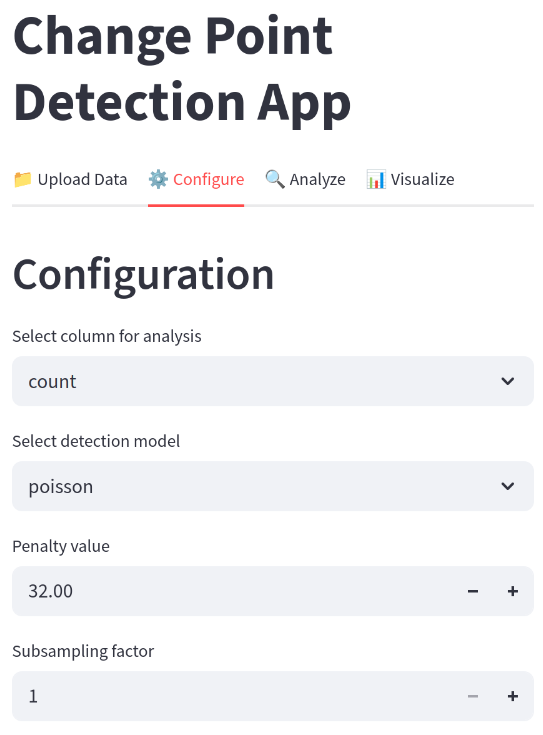
\includegraphics[width=\textwidth]{figures/changepoints-settings.png}
        \caption{Web app: settings}
        \label{fig:changepoints-settings}
    \end{subfigure}
    \hfill
    \begin{subfigure}{0.65\textwidth}
        \centering
        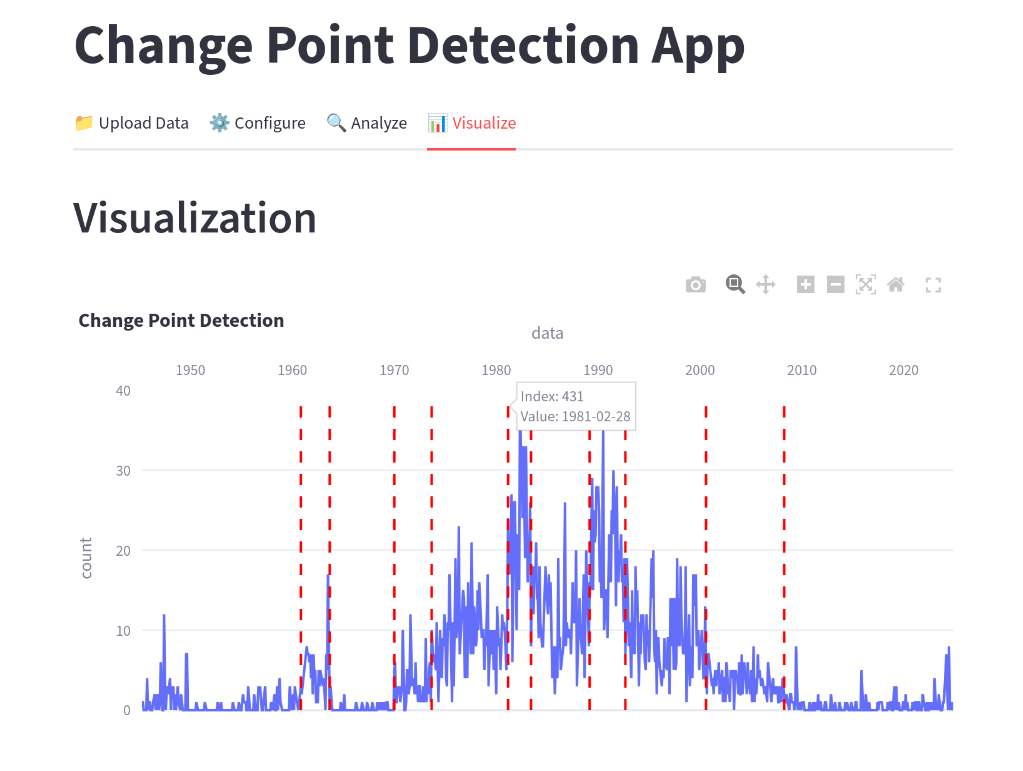
\includegraphics[width=\textwidth]{figures/changepoints.png}
        \caption{Web app: changepoint view}
        \label{fig:changepoints-webapp}
    \end{subfigure}
    \caption{
        Screenshots of the web application developed to visualize and explore the changepoint detection results. From the settings panel (\subref{fig:changepoints-settings}) it's possible to configure the algorithm parameters; the main view (\subref{fig:changepoints-webapp}) shows the time series of murders with detected changepoints in red dashed lines.
    }
    \label{fig:changepoints-webapp-full}
\end{figure}